% Describe why these models are useful. Show the ECN model... maybe something else.

\chapter{Application: ECN Hardening}

We considered the effects of network congestion on a cyber communication network used by the \ac{FREEDM} smart-grid, using a model of \ac{DGI} processes in a partitioned network.
By applying background traffic to the partitioned network, we create a situation where real-time deadlines are missed due to queuing delays.
In the \ac{FREEDM} smart-grid, the consequences of network congestion could result in several problematic scenarios.
First, if the congestion prevents \ac{DGI} from autonomously configuring using its group management system, processes cannot work together to manage power devices.
Secondly, if messages arrive too late, or are lost, the \ac{DGI} could apply settings to the attached power devices, driving the physical network to instability.
Unstable settings could lead to problems in the power-grid such as frequency instability, blackouts, and voltage collapse.
Congestion response techniques allow the DGI to anticipate behavior during a fault and allow it to harden itself against the fault.
In a smart-grid system, interfering traffic can originate from the use of public infrastructure at any level\cite{smartgrid-comm-germany}\cite{smartgrid-comm-lastmile}, a misconfigured device, changing networking requirements as new devices enter a network, or from an attacker in a \ac{DoS} attack.

\section{Theory of Operation}
In the simulated network, the router and the two switches were ECN enabled devices.
The devices monitored their incoming packet queues for each of their interfaces and used the \ac{RED} algorithm to determine when to mark a packet for \ac{ECN}.
Since \ac{ECN} fields in an IPv4 header are not directly available to an application, the notifications were multicast onto the source interface(s) of the packet that triggered the notification.
Each network device ran an application responsible for generating the multicast ECN message.

When the \ac{RED} algorithm identifies congestion, it must notify senders of congestion.
Because the approach is non-standard and most UDP applications would not understand the notification, we opted to create an application to run on switches and routers.
When congestion is detected, the application sends a multicast beacon to a group of interfaces informing the attached devices of the level of congestion.
For similarity with the \ac{RED} algorithm and the \ac{NS3} implementation, the notification is classified as either ``soft'' or ``hard.''
A soft notification is an indication the congestion in the network is approaching a level where real-time processes can expect message delays which may affect their normal operation.
A hard notification indicates the congestion has reached a level where messages are subject to both delay and loss.
%The notifications are rate limited so they do not flood the network.

\section{Group Management}

The group management module's execution schedule is broken into several periods of message generation and response windows.
Because the schedule of the \ac{DGI} is partially synchronous, the traffic generated by modules is bursty.
The number of messages sent is $O(n^2)$ (where $n$ is the number of processes in the system), in a brief window, dependent on how well the clocks are synchronized in the system.
The duration of the response window is dependent on the amount of time it takes for messages to propagate to the hardest-to-reach process.
Additionally, to contend with congestion, an additional slack must be added to allow the \ac{RED} algorithm to detect congestion before it reaches a critical level.
Figure \ref{fig:queue-types} depicts typical queuing behavior for a network device serving \ac{DGI} processes under different circumstances.

Because the traffic generated by \ac{DGI} modules is very bursty, there is a phenomenon where the bursty traffic mixed with steady background traffic causes the packet queue at the network device to fill.
With no background traffic, the impulse queues many messages, but those messages are distributed within real-time constraints.
When the background traffic is introduced, the queue takes longer to empty.
At a critical threshold, the queue does not empty completely before the next burst is generated by the \ac{DGI} and the services provided by \ac{DGI} are disrupted.
If the level of other traffic is sufficiently high, the queue completely fills, and no messages can be distributed.
The \ac{RED} algorithm and \ac{ECN} are used to delay or prevent the queue from reaching this critical threshold.

\begin{figure}
\centering
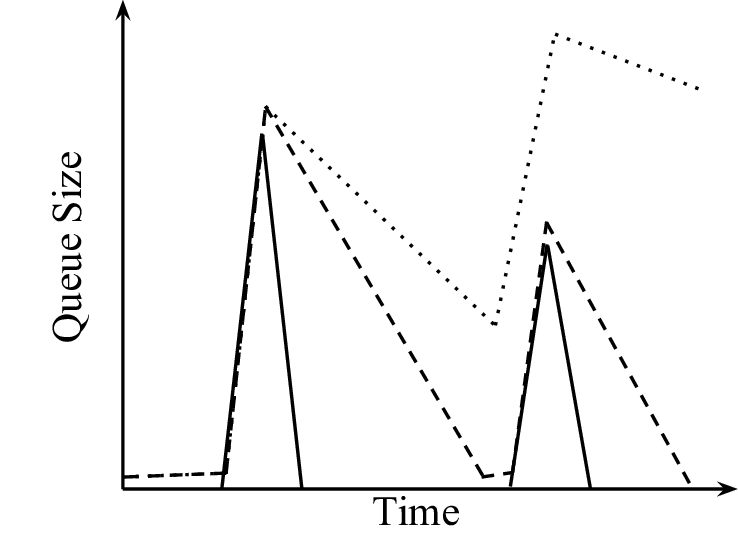
\includegraphics[width=0.4\linewidth]{QueueStacked}
\caption{
Example of network queuing during \ac{DGI} operation.
}
\ac{DGI} modules are semi-synchronous, and create bursty traffic on the network.
When there is no other traffic on the network (solid line), the bursty traffic causes many packets to queue quickly, but the queue empties at a similar rate.
With background traffic (dashed line), the bursty traffic causes many packets to be queued suddenly. More packets arrive continuously, causing the queue to drain off more slowly.
When the background traffic reaches a certain threshold (dotted line), the queue does not empty before the next burst occurs. When this happens, messages will not be delivered in time, and the queue may completely fill.
\label{fig:queue-types}
\end{figure}

\subsection{Soft \ac{ECN}}

A soft \ac{ECN} message indicates the network has reached a level of congestion where the router suspects processes will not be able to meet their real-time requirements.
The soft \ac{ECN} message encourages the \ac{DGI} processes to reduce the number of messages they send, reducing the amount of congestion they contribute to the network, and to allow for reliable distribution techniques to have additional time to deliver messages (since fewer messages are being sent).
In the case of potential congestion, the group management module can reduce its traffic bursts by disabling elections during the congestion.
When elections are disabled, messages for group management are only sent to members of the group.
Processes do not seek out better or other leaders with which to merge.
As a consequence, the message complexity for processes responding to the congestion notification reduces from $O(n^2)$ to $O(n)$.

\subsection{Hard \ac{ECN}}

In a hard \ac{ECN} scenario, the router will determine congestion has reached a threshold where the real-time processes will soon not be able to meet their deadlines.
In this scenario, the real-time process will likely split its group.
In an uncontrolled situation, the split will be random, and time will be wasted while the system is reorganizing.
It is, therefore, desirable when this level of traffic is reached to split the group.
Splitting the group reduces the number of messages sent across the router for modules with $O(n^2)$ (where $n$ is the number of processes in the original group) message complexity.
For larger groups, splitting them provides significant savings in the number of messages that must be queued by the router, especially since the traffic is very bursty.

\begin{figure}
\centering
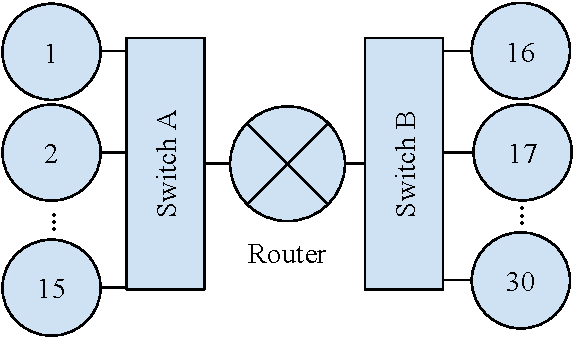
\includegraphics[width=0.35\textwidth]{NetworkLayout}
\caption[Example of process organization]{Example of process organization. Two groups of processes are connected by a router.} \label{fig:network-layout}
\end{figure}

Suppose a network like one depicted in Figure \ref{fig:network-layout}, where processes are divided by a router.
In Figure \ref{fig:network-layout}, there are $n$ processes on one side of the network and $m$ on the other.
In normal operation, the omission-modelable algorithm has an $O(n^2)$ message complexity.
In Soft \ac{ECN} maintenance mode, the reduced number of messages reduces the complexity to $O(n)$ by disabling elections.

During elections (and with each group update) the leader distributes a fallback configuration that will coordinate the division of the groups during intense congestion.
When the \ac{ECN} notification is received, the processes will halt all current group management operations and enter a splitting mode where they switch to the fallback configuration.
The leader of the group distributes a fallback notification to ensure all processes in the group apply their new configuration. 
The complexity of distributing the notification is linear $O(n)$ and processes that already received the notification will have halted their communication.
This approach will, ideally, avoid the burst/drain phenomena from Figure \ref{fig:queue-types}.

The design of the fallback configuration can be created to optimize various factors.
The factors include cyber considerations, such as the likely network path the processes in the group will use to communicate.
By selecting the group around cyber network resources, the group can be selected to minimize the amount of traffic that crosses the congested links in the future.
Additionally, considerations from the physical network can be considered.
Fallback groups can be created to ensure they can continue to facilitate the needs of the members.
The design of the configuration can take into the consideration the distribution of supply and demand processes in the current group.
By having a good mix of process types in the fallback group, the potential for work can remain high.

\section{Cyber-Physical System}

For a real-time \ac{CPS}, message delays could affect coordinated actions.
As a result, actions may not happen at the correct moments or at all.
Since the two-army problem prevents any process from being entirely certain a coordinated action will happen in concert, problems arising from delay or omission of messages is of particular interest.
Specifically, we are interested in the scenario from \cite{HARINI}, where only half of a power migration is performed.
Other power management algorithms could have similar effects on the power system based on this idea of a process performing an action that is not compensated for by other processes.

\subsection{Soft ECN Notification}

In a soft congestion mode, the process being informed of the congestion can reduce its effect on the congestion by changing how often it generates bursty traffic.
Processes running the load balancing algorithm make several traffic bursts when they exchange state information and prepare migrations.
As shown before, if the interval between these bursts is not sufficient for the queue to drain before the next burst occurs, then critical, overwhelming congestion occurs.
The schedule of the \ac{DGI} is fixed at run-time and processes cannot simply extend the duration of the load balancing execution phase.
However, on notification from the leader, the process can, instead, reduce the number of migrations to increase the message delivery interval.
The notification to reduce the schedule originates from the coordinator as part of the message exchange necessary for the process to remain in the group.
Every process in the group must receive the message to participate in load balancing, ensuring all processes remain on the same real-time schedule.
By using this approach, the amount of traffic generated is unchanged but the period a process waits for the messages to be distributed is increased.

\subsection{Hard ECN Notification}

When the \ac{DGI} process receives a hard congestion notification, the processes switch to a predetermined fallback configuration.
The configuration creates a cyber partition.
By partitioning the network, the number of messages sent by applications with $O(n^2)$ message complexity can be reduced significantly.
Each migration of the load balancing algorithm begins with an $O(n^2)$ message burst and so benefits from the reduced group size created by the partition.

Consider a network like the in Figure \ref{fig:network-layout} with $n$ processes on one half and $m$ on the other.
The number of messages sent across the router for the undivided group is of the order $2mn$ as the $n$ processes on side A send a message to the $m$ on side B and vice-versa.
Let $i_{1}$ and $j_{1}$ be the number of processes from side A and side B (respectively) in the first group created by the partition.
Let $i_{2}$ and $j_{2}$ be the number of processes in the second group created by the partition under the same circumstances of $i_1$ and $j_1$.
The number of messages sent that pass through the router, is then 

\begin{equation}
2 i_{1} j_{1} + 2 i_{2} j_{2}
\end{equation}

For an arbitrary group division, the following can be observed.
Suppose $i_{1}$ and $j_{2}$ are the cardinality of two arbitrarily chosen sets of processes from side A and side B respectively.
Following the same cut requirements as before:

\begin{equation}
i_2 = n - i_1 \text{ and } j_2 = m - j_1
\end{equation}

The number of messages that must pass through the router for this cut is:

\begin{equation}
2 i_{1} j_{1} + 2 (n-i_{1}) (m-j_{1})
\end{equation}

The benefits of the cut are minimized when $i_1$ and $j_1$ are $\frac{n}{2}$ and $\frac{m}{2}$:

\begin{equation}
2( 2 \frac{mn}{4} + mn - \frac{mn}{2} - \frac{mn}{2}) = mn
\end{equation}

Which is a reduction of half as many messages.
For systems with many participating processes, a significant reduction in the number of messages sent across the router is achieved.
As a consequence, this further extends the delivery window for processes sending messages by decreasing channel utilization.

\section{Relation To Omission Model}

The synchronization of clocks in the environment is assumed to be normally distributed around a true time value provided by the simulation.
The shape of the curve created by plotting the queue is \ac{CDF} of the normal distribution, noted $F(x)$.
A simple description of the traffic behavior can then be described in terms of that curve.
First, when the queue hits a specific threshold, even if the queue is drained at an optimal rate, the $n$th queued packed will not be delivered in time:

\begin{equation}
Qsize - min(Qsize, (DequeueRate * \Delta t)) \geq 0
\label{eq:origin}
\end{equation}

Where $\Delta t$ is the deadline for the message to be delivered.
If the size of the queue exceeds the number of messages that can be delivered before $\Delta t$ passes, some messages will not be delivered.
The size of the queue during the message bursts created by the DGI depends on the message complexity of the algorithm, the number of messages already in the queue, the other traffic on the network, and any replies needing to be delivered in that interval.
Therefore, let $c$ represent the rate traffic is generated by other processes.
Let $init_q$ represent the number of messages in the queue at the start of a burst. 
Let $init_m$ represent the number of messages sent in the beginning of the burst.
Let $resp$ represent the number of messages sent in response to the burst that must still be delivered before $\Delta t$ passes.
We can then express $Qsize$ as two parts:

\begin{equation}
Qsize = Burst + Obligations
\end{equation}

Where $Burst$ takes the form of the \ac{CDF} for the normal distribution:

\begin{equation}
Burst = init_m * F(x)  
\end{equation}

\begin{equation}
Obligations = c * \Delta t + init_q + resp
\end{equation}

From this we can derive the equation:

\begin{equation}
F(x) \geq \frac{DequeueRate * \Delta t - c * \Delta t - init_q - resp}{init_m}
\label{eq:prob-est}
\end{equation}

Where, from Equation \ref{eq:origin}, $DequeueRate * \Delta t$ is less than or equal to the number of messages in the queue. 
Solving for $F(x)$ gives a worst case estimate of the omission rate for a specific algorithmic or network circumstance.
$DequeueRate$ is affected by the amount of traffic in the system. 
It should be noted, a greater amount of background traffic corresponds to a greater average queue size.
From an relationship between the background traffic and the average queue size and the results presented in \cite{JOURNAL}, Equation \ref{eq:prob-est} can be used to select the ECN parameters.

%   - Show the unbounded Queue Graph and the mess it makes of LB and GM
%   - Show soft ECVN allows more work to be done, possibly at the cost of accumulating K.
%   - Shwo that HARD ecn allows the best operation -- work gets done and less K is accumlated.

% Show a control. 
% Normal operation. Highlight the bursty peaks from the \ac{DGI} algorithm running
% Point out the average queue size as a second line.
% State a relationship between the average queue size and the message delay.

% Introduce a sufficent amount of traffic to make the queue drain off slowly, recreating the previous figure
% State again that as the amount of other traffic increases the time to drain the queue starts to increase
% State that this does not affect normal operation because the \ac{DGI} has slack built into the schedule to ensure that a normal amount of background traffic does not cripple the \ac{DGI}.
% State that as the traffic increases further, eventually it will over flow the queue
% Show the unbounded queue growth for a drop tail queue.

% Introduce the \ac{RED} queue.
% Show that the \ac{RED} queue, without notifying the \ac{DGI} can do some management, but it isn't sufficent to keep the groups together.
% Show that based on the control, less work gets done and the groups change more frequently.

% Introduce the \ac{ECN} notification
% If the \ac{RED} queue allows \ac{DGI} traffic to pass (making the \ac{RED} queue more like a drop-tail for \ac{DGI} traffic) show that it improves on the previous scenario.
% Show that however, eventually the traffic reaches a threshold where the stratedgy is not sufficent to prevent issues.
% Introduce the \ac{DGI} reacting to the notifications.
% Show that when the \ac{DGI} goes into a maintain mode the average traffic drops.
% Show that this allows a large group to be maintained and the migrations to proceed as normal (with the time reduced schedule).

% Introduce HARD groupbreaks.
% Show that a hard group break greatly reduces traffic (even more than previously) & that this allows the \ac{DGI} to determine how to split.
% Demonstrate a worst-case scenario where the group break is not optimal.
% Show that a planned hard break allows that group to continue operating.

\section{Proof Of Concept}

\subsection{Experimental Setup}
\label{sect:experimentalsetup}

Experiments were run in a Network Simulator 3.23\cite{NS3} test environment.
The simulation time replaced the wall clock time in the \ac{DGI} for the purpose of triggering real-time events.
As a result, the computation time on the \ac{DGI} for processing and preparing messages was neglected.
However, to compensate for the lack of processing time, the synchronization of the \ac{DGI} was randomly distributed as a normal distribution.
This was done to introduce realism to ensure events did not occur simultaneously.
Additionally, the real-time schedules used by the \ac{DGI} were adjusted to remove the processing time that was neglected in the simulation.
The schedule used is depicted in Figure X.

The \ac{DGI} were placed into a partitioned environment.
The test included 30 nodes.
Each of the nodes ran one \ac{DGI} process.
Two sets of 15 \ac{DGI} were each connected to a switch and each switch was in turn connected to the router.
The network is pictured in Figure \ref{fig:network-layout}.
Node identifiers were randomly assigned to nodes in the simulation and used as the process identifier for the \ac{DGI}.
In the experiments the load at each process was randomly assigned: each side is mix of supply and demand processes.

The links between the router and the switches had a \ac{RED} enabled queue placed on both network interfaces.
The \ac{RED} parameters for all queues were set identically.
A summary of \ac{RED} parameters are listed in Table \ref{tab:red-parameters}.
All links in the simulation were 100Mbps links with a 0.5ms delay.
RED was used in packet count mode to determine congestion.
ARP tables were populated before the simulation began.
\ac{RED} parameters were selected using results from \cite{JOURNAL}.

The relationship between the background traffic and the average queue size was estimated through runs of the \ac{NS3} simulation.
Figure \ref{fig:plotm} demonstrates the observed relationship between the total background traffic and the maximum average queue size for that level of traffic.
Additionally, the $DequeueRate$ was collected from a run of the simulation without traffic, and was found to be $713.08$ packets/second.
Therefore, from Equation \ref{eq:prob-est}, assuming $init_q=0, resp=225, init_m=225$ and $\Delta t=1$, the maximum traffic rate with no omissions was $263.0$ packets/second.
The number of packets for the $resp$ and $init_m$ were selected from the worst case of the algorithm in \cite{JOURNAL}.
Based on the traffic parameters in Table \ref{tab:red-parameters}, $263.0$ packets/second corresponded to 1.077 Mbps of traffic generated at one switch and 2.1545 Mbps traffic overall.
From the polynomial estimate in Figure \ref{fig:plotm}, the maximum average queue size for that level of traffic was $94.715$, estimated as $90$ for the \ac{RED} Min Threshold in Table \ref{tab:red-parameters}.
RED Max Threshold is computed using a similar technique, but using the message complexity for the Load Balancing algorithm, since it maintained its complexity during Soft ECN mode.

\begin{figure}
\centering
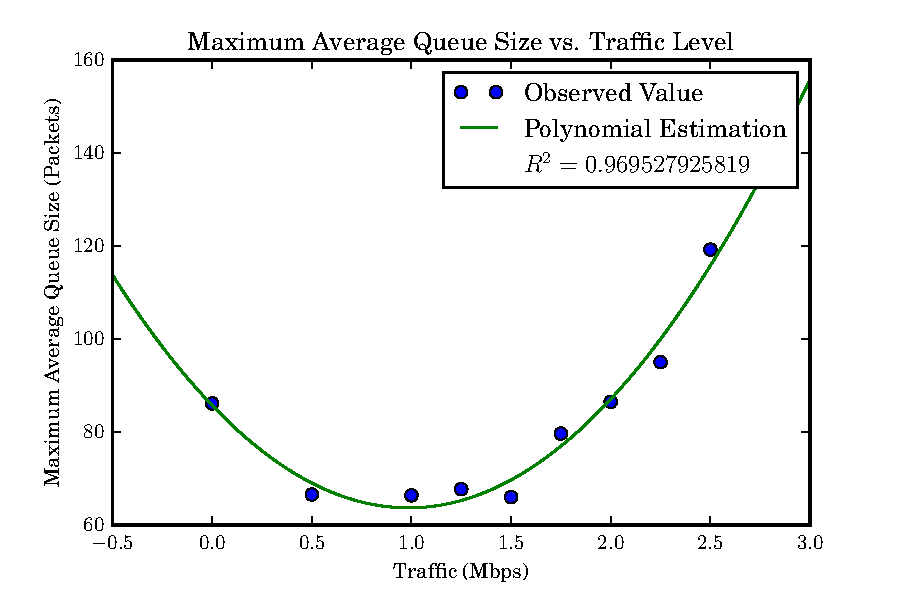
\includegraphics[width=0.65\linewidth]{m-max-average-queue.pdf}
\caption[Plot of the maximum observed average queue size as a function of the overall background traffic.]{Plot of the maximum observed average queue size as a function of the overall background traffic. The polynomial estimate is $y=22.70x^2-44.74x+85.72$}
\label{fig:plotm}
\end{figure}

\begin{table}
\begin{center}
\begin{tabular}{ | l | l || l | l | } \hline
Parameter & Value & Parameter & Value        \\ \hline
RED Queueing Mode & Packet & RED Gentle Mode & True    \\ \hline
RED $Q_{w}$ & 0.002 & RED Wait Mode & True      \\ \hline
RED Min Threshold & 90 & RED Max Threshold & 130   \\ \hline
%Maximum Queue Size & 1000 \\ \hline
RED Link Speed & 100 Mbps & RED Link Delay & 0.5 ms   \\ \hline
%Clock Distribution $\sigma$ & 0.005 & Traffic Packet Size & 512 Bytes \\ \hline
\end{tabular}
\end{center}
\caption{Summary of \ac{RED} parameters. Unspecified values default to the \ac{NS3} implementation default value}
\label{tab:red-parameters}
\end{table}

To introduce traffic, processes attached to each of the switches attempted to send a high volume of messages to each other across the router.
The number of packets sent per second was a function of the data rate and the size of the packets sent.
In each simulation, half of the traffic originated from each switch.
Due to the properties of the network links, the greatest queueing effect occurred at the switches.

\subsection{Average Case Results}
\label{sect:results}
Six test scenarios were created to evaluate the \ac{ECN} technique.
The six scenarios are summarized in Table \ref{tab:scenarios}.
In each scenario, the distribution of supply and demand processes is mixed: each switch has a mix of supply and demand processes.
The potential of the system to complete migrations, as well as the potential for migrations to fail were primary considerations for each scenario.
Processes cannot initiate migrations if they are not grouped with other processes.
Similarly, if the process is attempting to communicate over a congested link, it may not meet real-time deadlines or successfully complete migrations.

\begin{table}
\centering
\caption{Summary of Scenarios Run}
\begin{tabular}{| c | c | c | c |}
    \hline
    Test & Traffic & Notifications & Attempted Migrations \\ \hline
    A & None & N/A & 1171 \\ \hline
    B & 2Mbps & N/A & 1171 \\ \hline
    C & 4Mbps & None & 1114  \\ \hline
    D & 4Mbps & Soft & 888 \\ \hline
    E & 6.4Mbps & Soft & 861 \\ \hline
    F & 6.4Mbps & All & 888 \\ \hline
\end{tabular}
\label{tab:scenarios}
\end{table}

Figures \ref{fig:plota} and \ref{fig:plotb} (Scenario A) show the normal operation of the system.
In this configuration, there is no congestion on the network. 
The \ac{DGI} start, group together and then begin migrating power between processes.
Figure \ref{fig:plota} plots the queue size over time for a queue used to send packets from a switch to the router.
Figure \ref{fig:plotb} is a detailed view of a portion of Figure \ref{fig:plota}.
Figure \ref{fig:plotb} shows the queue size during the normal operation of group management as well as the first three migrations of a load balancing round.
The dotted line plots the \ac{EWMA} of the size of the queue.
An important note for the plotted \ac{EWMA} values: \ac{NS3} only updates the average queue size during simulation when a new packet is enqueued.
As a consequence, the average queue size is slightly misleading the in scenarios where there is a significant amount of idle channel time (such as Figures \ref{fig:plota}, \ref{fig:plotb}, and \ref{fig:plote}).
In scenarios A and B, the traffic is not sufficient to disrupt the operation of the DGI.
As a result, in Figure \ref{fig:groupstatedistro}, process 0 has an uninterrupted observation of a group size of 30 throughout the two scenarios.

\begin{figure}
\centering
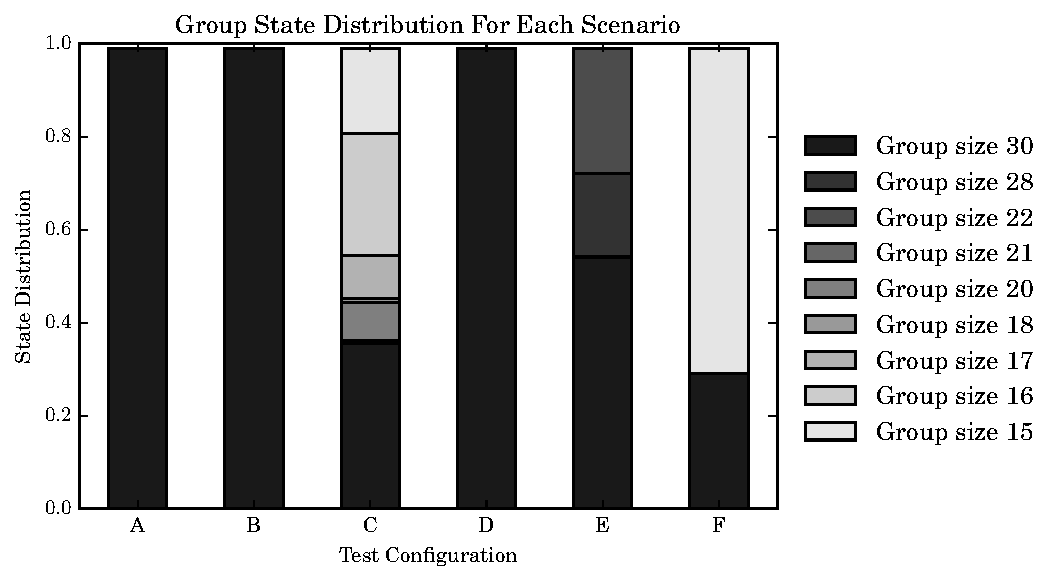
\includegraphics[width=0.95\textwidth]{groupstatedistribution.pdf}
\caption[Distribution of group sizes for process 0 in each scenario.]{Distribution of group sizes for process 0 in each scenario. The list of scenarios is presented in \ref{tab:scenarios}.  The height of each colored segment indicates the portion of the simulation where process 0 was in the given configuration.}
\label{fig:groupstatedistro}
\end{figure}

\begin{figure}
\centering
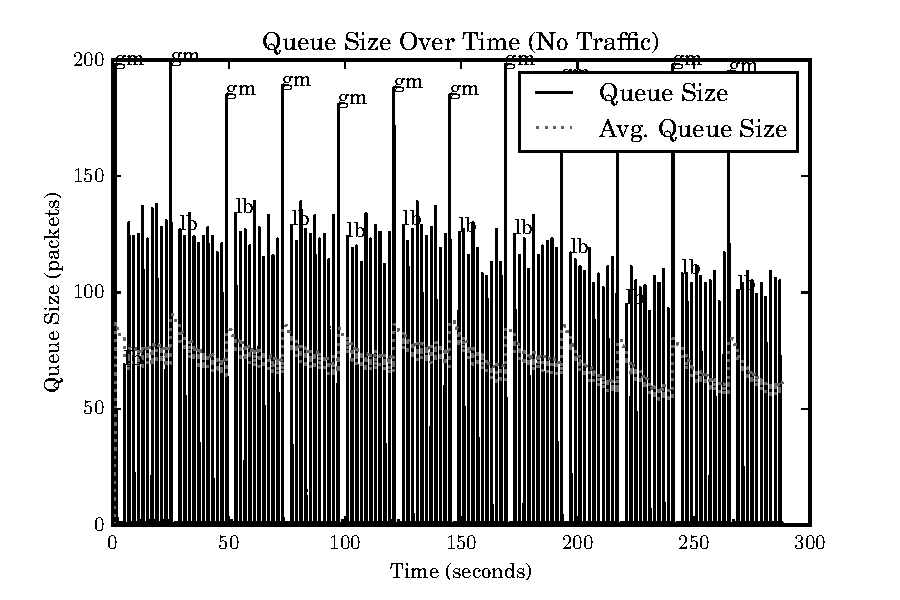
\includegraphics[width=0.75\textwidth]{a-qsizeot-notraffic-all.pdf}
\caption{Plot of the queue size for a queue from switch A to the router when only the DGI generates traffic.}
\label{fig:plota}
\end{figure}

\begin{figure}
\centering
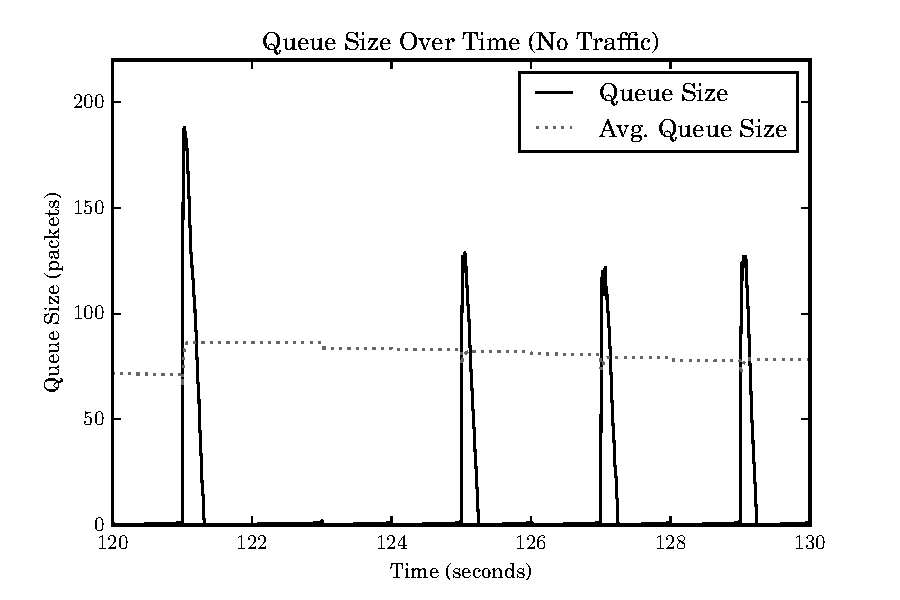
\includegraphics[width=0.75\textwidth]{b-qsizeot-notraffic-120s-130s.pdf}
\caption[Detailed view of Figure \ref{fig:plota}.]{
Detailed view of Figure \ref{fig:plota}. In the figure, the dark gray section is the period where the group management module executes.
The alternating white and light gray sections are the execution periods for individual migrations.
In the normal schedule, the DGI allocates approximately 1 second to each migration and performs 10 migrations each round.
Three migrations are shown in the figure.}
\label{fig:plotb}
\end{figure}

\begin{figure}
\centering
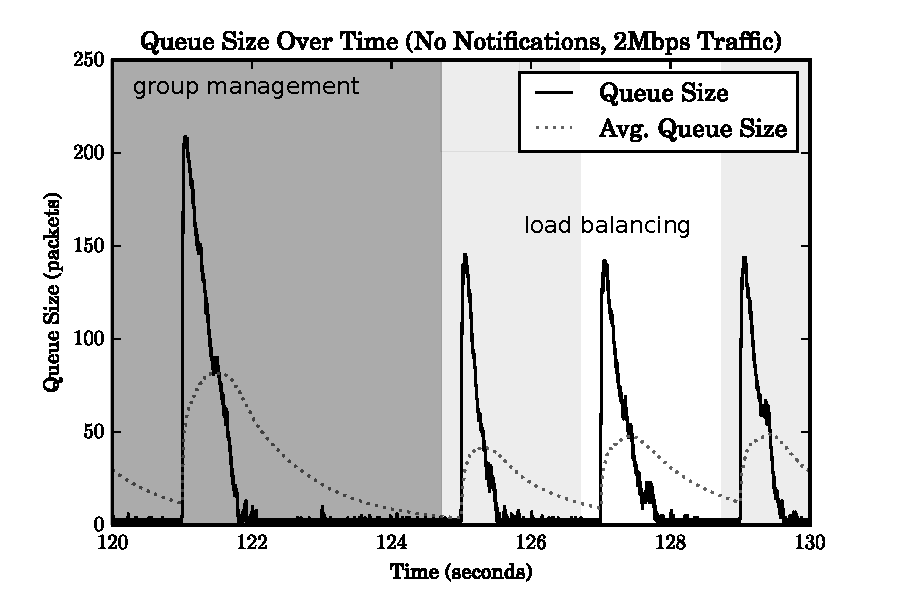
\includegraphics[width=0.75\textwidth]{e-qsizeot-nonotifications-2mbpstraffic-120s-130s.pdf}
\caption[Detailed view of the effect on queue size as other network traffic is introduced.]{
Detailed view of the effect on queue size as other network traffic is introduced.
Compared to Figure \ref{fig:plotb}, the peaks are taller and wider. 
The background traffic creates the intermediate effect described in \ref{fig:queue-types}.
As with Figure \ref{fig:plotb}, this figure shows 3 migrations.}
\label{fig:plote}
\end{figure}

\begin{figure}
\centering
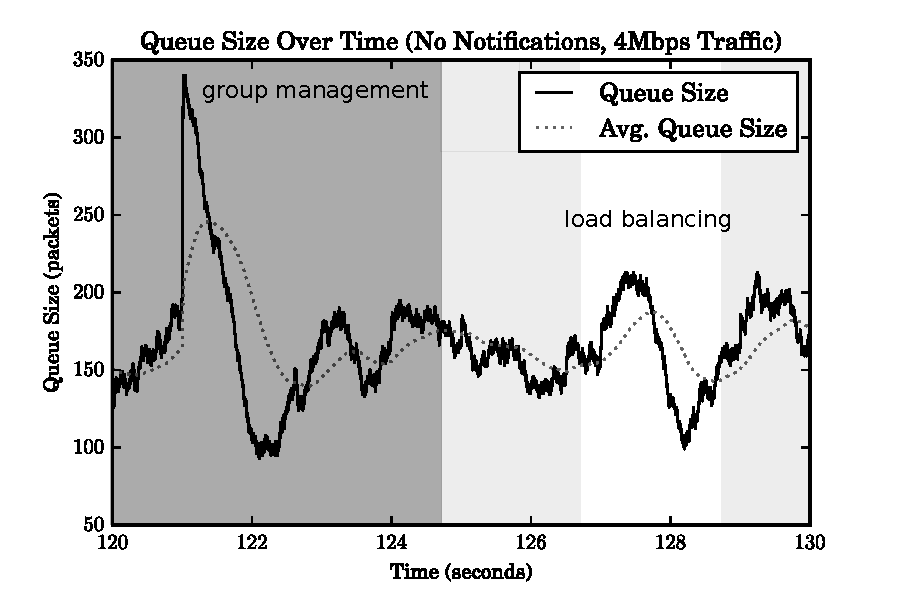
\includegraphics[width=0.75\textwidth]{f-qsizeot-nonotifications-4mbpstraffic-120s-130s.pdf}
\caption[Detailed view of the effect on queue size as other network traffic is introduced without notifications.]{
Detailed view of the effect on queue size as other network traffic is introduced without notifications.
In this scenario, the queue does not empty completely before the next burst of traffic occurs.
As a result, Group Management generates a large peak as it tries to rejoin groups that have broken due to the message delays.
Load balancing has smaller and less pronounced peaks because the groups are smaller.
Additionally, during this scenario some migrations are lost due to message delays.}
\label{fig:plotf}
\end{figure}

From scenario A and B we establish the $min_{th}$ value used as a \ac{RED} queue parameter.
The traffic generated by each step of the group management algorithm is very bursty.
The tightness of the clock synchronization in the group affect the size of the peak.
Like \cite{HILTESTBED}, the level of power at a process is the net sum of its power generation capability and load.
As power is shared on the network, processes with excess generation, converge toward zero net power.
Demand processes also converge toward zero net power.

\begin{figure}
\centering
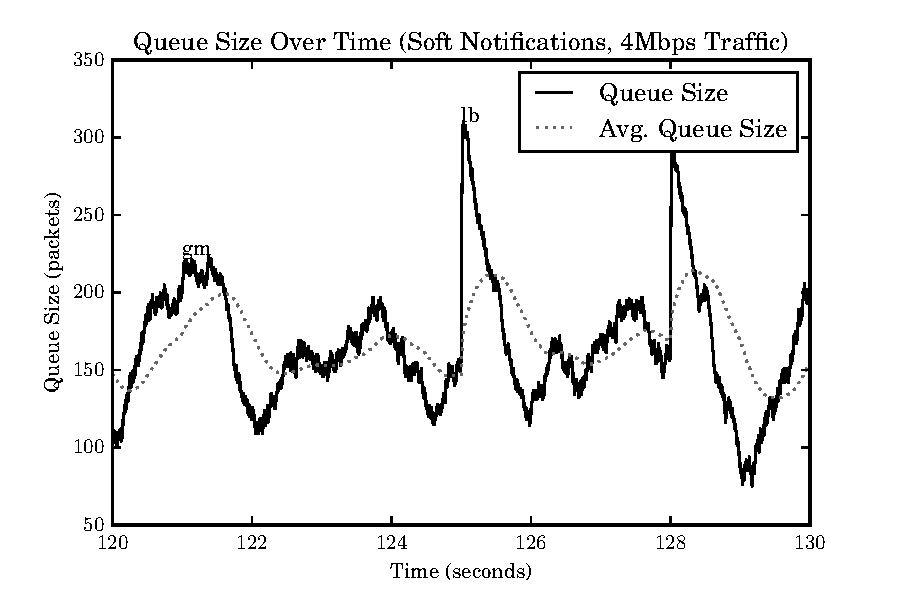
\includegraphics[width=0.75\textwidth]{i-qsizeot-softnotifications-4mbpstraffic-120s-130s.pdf}
\caption[Detailed view of the effect on queue size as other network traffic is introduced with soft \ac{ECN} notifications.]{
Detailed view of the effect on queue size as other network traffic is introduced with soft \ac{ECN} notifications.
In this scenario, the group management module entered a maintenance mode where it suspended discovering leaders of other groups.
As a result, that module's message complexity dropped significantly, resulting in the lack of a noticeable peak compared to previous scenarios.
Additionally, the system decreased the number of migrations performed per round by load balancing.
As a consequence, only two migrations are pictured.
Load balancing has higher peaks than in Figure \ref{fig:plotf} because groups have not been disbanded.
However, the reduced schedule is sufficient to prevent any migrations from being lost.
}
\label{fig:ploti}
\end{figure}

\begin{figure}
\centering
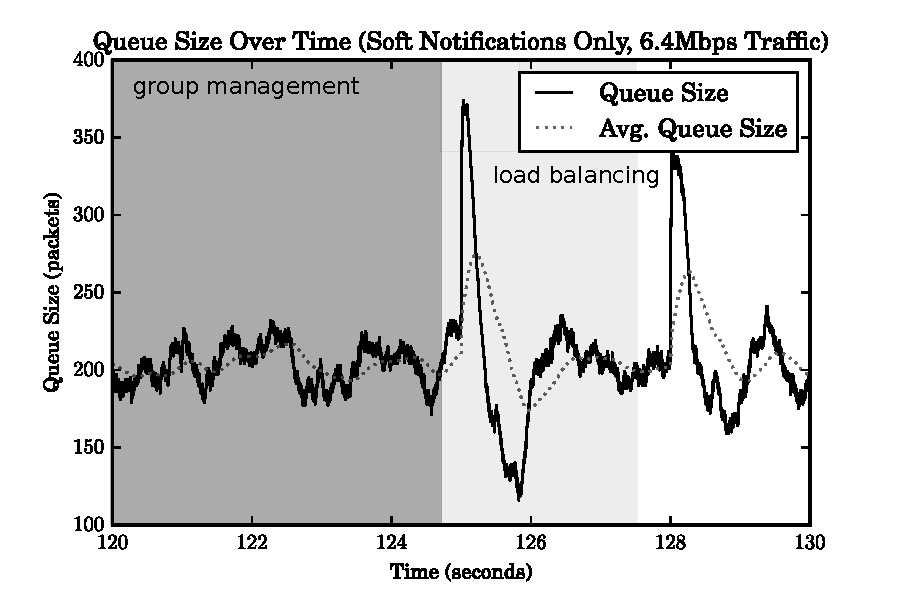
\includegraphics[width=0.75\textwidth]{k-qsizeot-softnotificationsonly-64mbpstraffic-120s-130s.pdf}
\caption[Detailed view of the effect on queue size as a large amount network traffic is introduced.]{
Detailed view of the effect on queue size as a large amount network traffic is introduced.
In this scenario, group management enters a maintenance mode when it receives the soft \ac{ECN} notification, but that approach alone is not sufficient to maintain groups: processes leave the group randomly during the simulation.
The system decreased the number of migrations per round, as it had done in \ref{fig:ploti}.
However, migrations were lost.
}
\label{fig:plotk}
\centering
\end{figure}

\begin{figure}
\centering
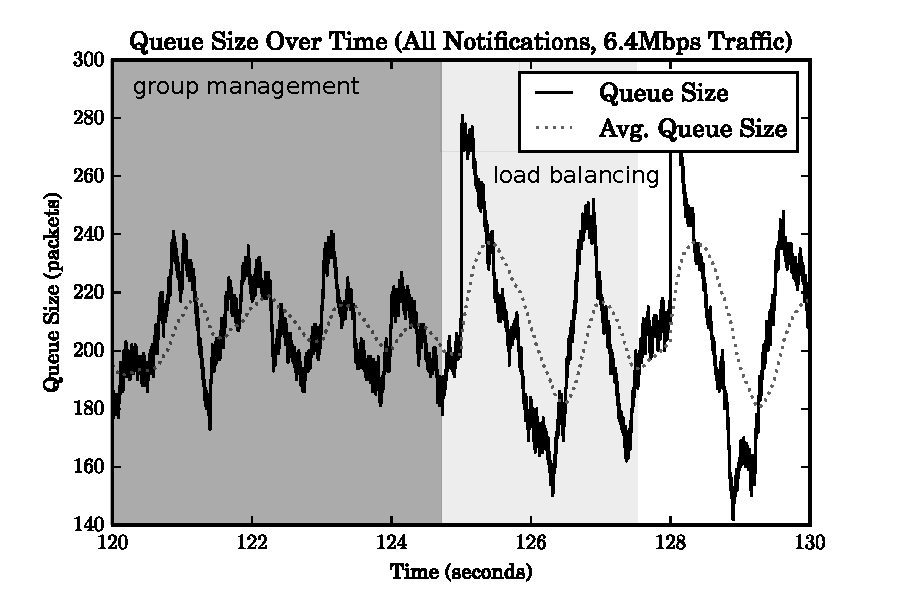
\includegraphics[width=0.75\textwidth]{l-qsizeot-allnotifications-64mbpstraffic-120s-130s.pdf}
\caption[Effect on queue size as a large amount of network traffic is introduced.]
{
In this scenario, hard notifications caused the groups to perform a coordinated division, enabled maintenance mode for the group management modules, and reduced the migration schedule for the load balancing module.
As a consequence, the group management module produced more traffic than it did in \ref{fig:plotk}, but, the installed fallback configurations did not have any of the \ac{DGI} leave the group.
Additionally, the smaller group size allowed the amount of traffic from the load balancing module to be reduced while still allowing the module to migrate power between \ac{DGI} without any migrations being lost.
}
\label{fig:plotl}
\end{figure}

\begin{figure}
\centering
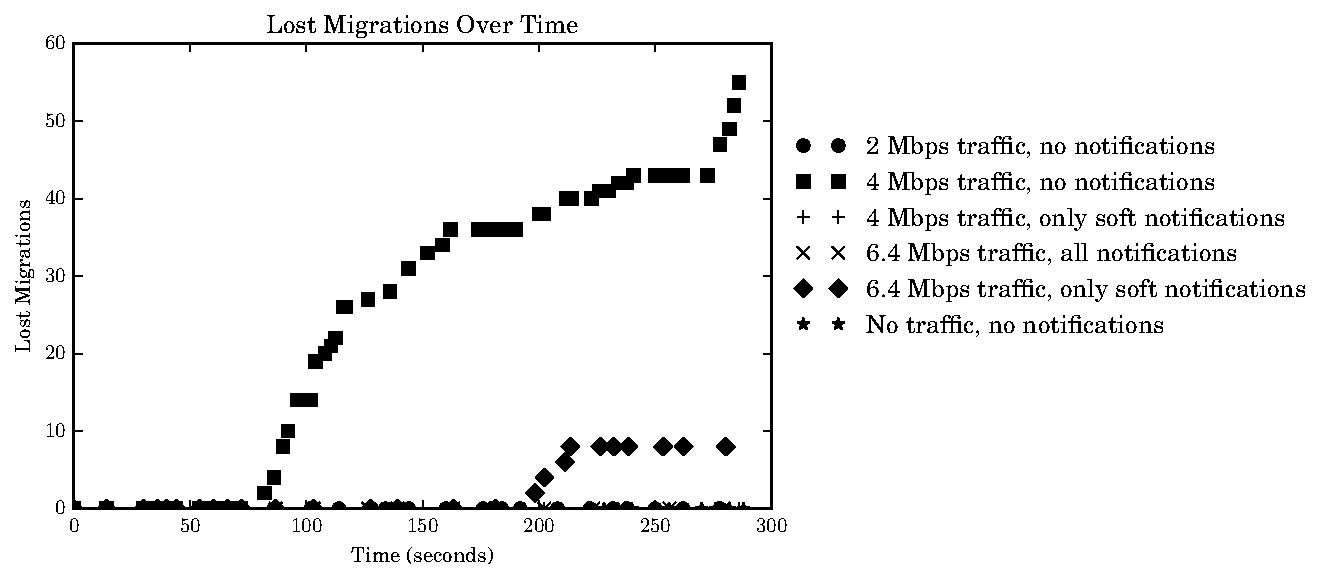
\includegraphics[width=0.95\textwidth]{failedmigrations.pdf}
\caption[Count of lost migrations from all processes over time.]{Count of lost migrations from all processes over time. Migrations are counted as lost until the second process confirms it has been completed. Without congestion management, migrations are lost.}
\label{fig:plotg}
\end{figure}

Figure \ref{fig:plote} shows the queue size as the network traffic begins to increase.
The \ac{DGI} in these experiments used schedule that allowed for some congestion to occur before processes are disrupted.
The slack gave network devices the opportunity to identify when the network congestion would go beyond the acceptable threshold.

Figure \ref{fig:plotf} (Scenario C) shows an example of congestion affecting the physical network without \ac{ECN}.
As a result of the congestion in Figure \ref{fig:plotf}, processes leave the main group, shown in \ref{fig:groupstatedistro}.
The observed configurations have greater than 15 processes because communication that does not cross the switch-router-switch path is not congested.
As a consequence, processes on the same switch as process 0 do not leave 0's group.
Power migrations are affected by congestion: migrations fail, or the supply process is left uncertain of migrations completions.
Figure \ref{fig:plotg} plots the count of failed migrations over time.
The number of failed migrations relative to the number attempted is quite low, because processes on the same switch as process 0 can still attempt migrations.

%In this scenario, only migrations are completed compared to the control.

Figure \ref{fig:ploti} (Scenario D) shows an example of the \ac{ECN} algorithm notifying processes of the congestion.
Compared to the scenario in Figure \ref{fig:plotf} (Scenario C), the \ac{ECN} algorithm successfully prevents the group from dividing.
As part of the compensation for the congestion, the number of migrations attempted are reduced, as listed in Table \ref{tab:scenarios}.
In \cite{ecn-cloudhari}, when the number of migrations are reduced, the size of each migration is increased.
Despite fewer migrations being attempted, the same amount of power can be managed by the \ac{DGI}, and the number lost migrations is reduced by the changed schedule.

Figures \ref{fig:plotk} (Scenario E) and \ref{fig:plotl} (Scenario F) show an example of a more extreme congestion scenario.
In Figure \ref{fig:plotl}, the \ac{RED} algorithm shares a Hard \ac{ECN} notification.
The notification causes the \ac{DGI} to switch to a smaller fallback configuration and fallback configuration decreases the queue usage from Figure \ref{fig:plotk} to Figure \ref{fig:plotl}.
Without this fallback configuration behavior, the system is greatly affected by the traffic.
However, with the fallback configuration the system remains stable and no migrations are lost.

\subsection{Worst Case Results}

In the worst case, supply processes and demand processes are not intermixed at each switch: only supply processes are at switch A, and only demand processes are at switch B.
The placement of processes is the worst case because it involves the highest number of messages crossing the congested link.
No migration can occur without messages crossing the congested link.
As a result, in the worst case scenarios, hard \ac{ECN} messages are triggered at a lower level of traffic than in the average case scenarios.
This is expected: in soft \ac{ECN} mode, the majority of traffic comes from the load balancing algorithm and in the worst case, the load balancing algorithm can only perform migrations while using the congested link.
A summary of test scenarios for the worst case is presented in \ref{tab:scenarios-worst}.

\begin{table}
\centering
\caption{Summary of Scenarios Run}
\begin{tabular}{| c | c | c | c |}
    \hline
    Test & Traffic & Notifications & Attempted Migrations \\ \hline
    G & 4Mbps & None &  \\ \hline
    H & 4Mbps & Soft &  \\ \hline
    I & 5.1Mbps & Soft & \\ \hline
    J & 5.1Mbps & All &  \\ \hline
\end{tabular}
\label{tab:scenarios-worst}
\end{table}

Figure X shows the number of lost migrations for each scenario.
Because all migrations must be completed with the congested link, there is a greater number of failed migrations and the number of migrations attempted is reduced because of the congestion (Scenario G).
The queue size for Scenario G is presented in Figure Y.
Enabling soft ECN mode (Scenario H), as before, prevents failed migrations.
Scenario G's queue is presented in figure Z.

The hard ECN message is triggered earlier in the worst case, due to the increased dependence on the congested link.
Figure ZA shows the queue size for Scenario I, a scenario that should trigger hard ECN mode.
In Scenario I, uncontrolled group division occur and migrations are lost.
By enabling notifications (Scenario J) those situations are mitigated.
